\section{Les Fonctions - Principe et généralités}

\begin{frame}{Les Fonctions - Principe et généralités}

\begin{itemize}[label=\textbullet, font= \color{greenperso}]
    \item Utiles pour réaliser plusieurs fois la même opération au sein d'un programme. 
    \item Elles rendent également le code plus lisible et plus clair en le fractionnant en blocs logiques.
\end{itemize}
\end{frame}


\begin{frame}{Les Fonctions natives Python}
    

Vous connaissez déjà certaines fonctions Python. Par exemple des fonctions internes à Python comme :

\begin{itemize}[label=\textbullet, font= \color{greenperso}]
    \item range() : indication pour effectuer une action un certain nombre de fois dans une boucle for
    \item len() : donner la taille d'une liste, d'une chaîne de caractères
    \item print() : affichage
    \item type() : type de la valeur 
\end{itemize}
\end{frame}



\begin{frame}{Les Fonctions}
Pour l'instant, une fonction est à vos yeux une sorte de « boîte noire » (voir figure 1) :
\begin{itemize}[label=\textbullet, font= \color{greenperso}]
    \item À laquelle vous indiquez aucune, une ou plusieurs variable(s) entre parenthèses. Ces variables sont appelées \textbf{arguments}. Il peut s'agir de n'importe quel type d'objet Python.

 \item Qui effectue une action.
\item Et qui renvoie un objet Python ou rien du tout.
\end{itemize}
\end{frame}


\begin{frame}{Les Fonctions}

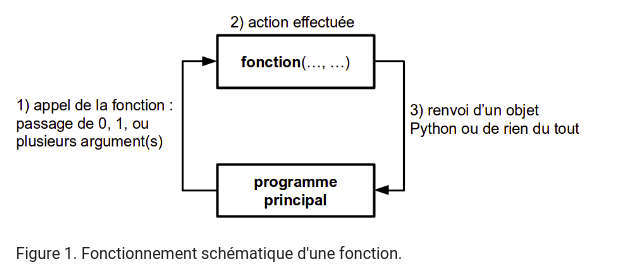
\includegraphics[scale=0.5]{images/fonctions.png}
    
\end{frame}

\section{Déclarer et appeler une fonction}

\begin{frame}{Les Fonctions}

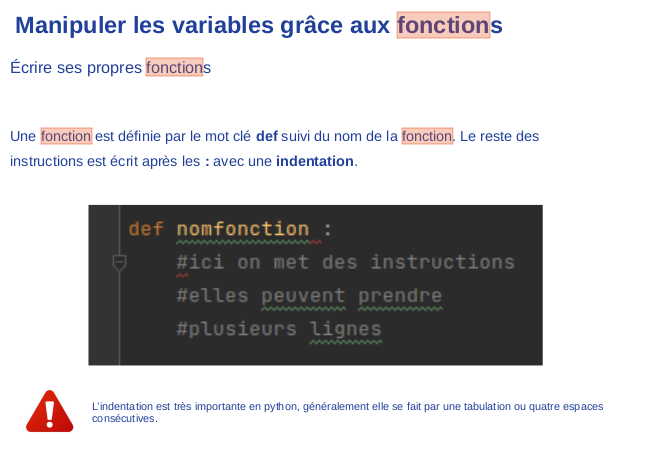
\includegraphics[scale=0.5]{images/fonction_2.png}
    
\end{frame}

\begin{frame}{Les Fonctions}

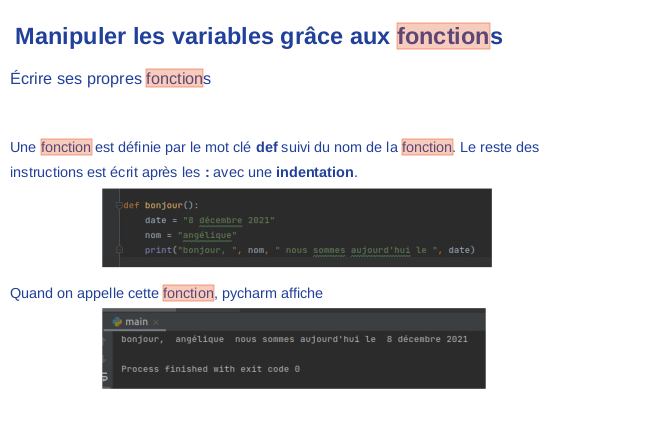
\includegraphics[scale=0.5]{images/fonctions_3.png}
\vspace{-0.3cm}
\footnotesize{$*$ \textit{pycharm} est un IDE, au même titre que \textit{Spyder ou Jupyter notebook}...}
    
\end{frame}

\begin{frame}{Les Fonctions}

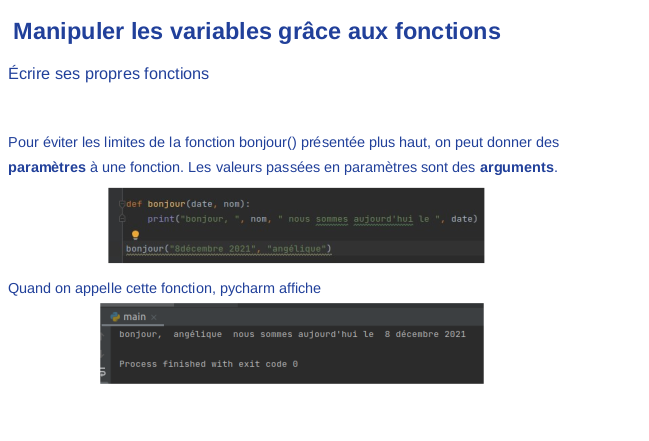
\includegraphics[scale=0.5]{images/fonction_3.png}
\vspace{-0.3cm}
\footnotesize{$*$ \textit{pycharm} est un IDE, au même titre que \textit{Spyder ou Jupyter notebook}...}
    
\end{frame}

\begin{frame}{Les Fonctions}

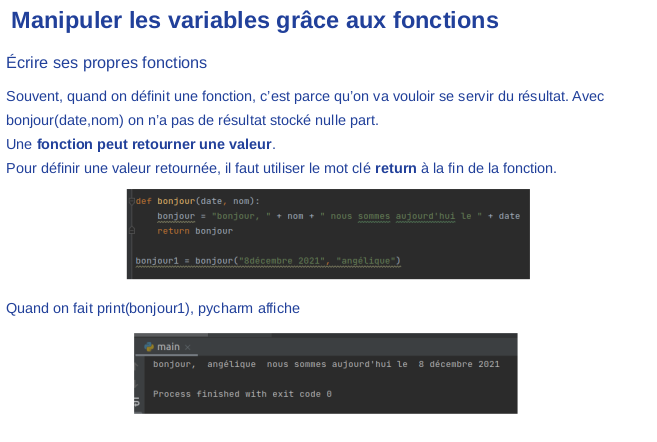
\includegraphics[scale=0.5]{images/fonction-4.png}
    
\end{frame}

\begin{frame}{Les Fonctions}

Exercice :
Écrire une fonction qui retourne l’endroit où nous sommes actuellement et ce que nous faisons en utilisant des paramètres
    
\end{frame}


\begin{frame}{Les Fonctions}
Ecrire la fonction 
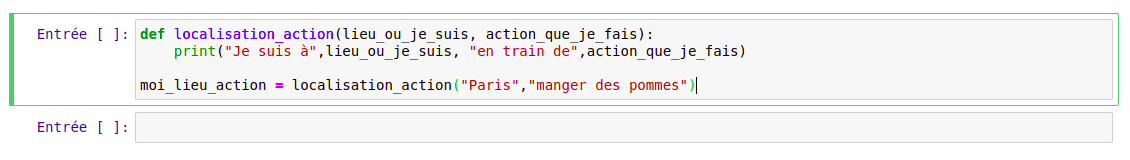
\includegraphics[scale=0.3]{images/fonction_1.png}
\pause

\vspace{1cm}
Quand on fait tourner le programme on obtient : 
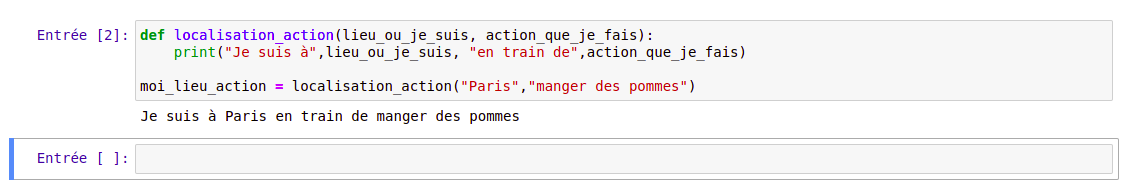
\includegraphics[scale=0.3]{images/fonction2.png}

\end{frame}
